\documentclass[1p]{elsarticle_modified}
%\bibliographystyle{elsarticle-num}

%\usepackage[colorlinks]{hyperref}
%\usepackage{abbrmath_seonhwa} %\Abb, \Ascr, \Acal ,\Abf, \Afrak
\usepackage{amsfonts}
\usepackage{amssymb}
\usepackage{amsmath}
\usepackage{amsthm}
\usepackage{scalefnt}
\usepackage{amsbsy}
\usepackage{kotex}
\usepackage{caption}
\usepackage{subfig}
\usepackage{color}
\usepackage{graphicx}
\usepackage{xcolor} %% white, black, red, green, blue, cyan, magenta, yellow
\usepackage{float}
\usepackage{setspace}
\usepackage{hyperref}

\usepackage{tikz}
\usetikzlibrary{arrows}

\usepackage{multirow}
\usepackage{array} % fixed length table
\usepackage{hhline}

%%%%%%%%%%%%%%%%%%%%%
\makeatletter
\renewcommand*\env@matrix[1][\arraystretch]{%
	\edef\arraystretch{#1}%
	\hskip -\arraycolsep
	\let\@ifnextchar\new@ifnextchar
	\array{*\c@MaxMatrixCols c}}
\makeatother %https://tex.stackexchange.com/questions/14071/how-can-i-increase-the-line-spacing-in-a-matrix
%%%%%%%%%%%%%%%

\usepackage[normalem]{ulem}

\newcommand{\msout}[1]{\ifmmode\text{\sout{\ensuremath{#1}}}\else\sout{#1}\fi}
%SOURCE: \msout is \stkout macro in https://tex.stackexchange.com/questions/20609/strikeout-in-math-mode

\newcommand{\cancel}[1]{
	\ifmmode
	{\color{red}\msout{#1}}
	\else
	{\color{red}\sout{#1}}
	\fi
}

\newcommand{\add}[1]{
	{\color{blue}\uwave{#1}}
}

\newcommand{\replace}[2]{
	\ifmmode
	{\color{red}\msout{#1}}{\color{blue}\uwave{#2}}
	\else
	{\color{red}\sout{#1}}{\color{blue}\uwave{#2}}
	\fi
}

\newcommand{\Sol}{\mathcal{S}} %segment
\newcommand{\D}{D} %diagram
\newcommand{\A}{\mathcal{A}} %arc


%%%%%%%%%%%%%%%%%%%%%%%%%%%%%5 test

\def\sl{\operatorname{\textup{SL}}(2,\Cbb)}
\def\psl{\operatorname{\textup{PSL}}(2,\Cbb)}
\def\quan{\mkern 1mu \triangleright \mkern 1mu}

\theoremstyle{definition}
\newtheorem{thm}{Theorem}[section]
\newtheorem{prop}[thm]{Proposition}
\newtheorem{lem}[thm]{Lemma}
\newtheorem{ques}[thm]{Question}
\newtheorem{cor}[thm]{Corollary}
\newtheorem{defn}[thm]{Definition}
\newtheorem{exam}[thm]{Example}
\newtheorem{rmk}[thm]{Remark}
\newtheorem{alg}[thm]{Algorithm}

\newcommand{\I}{\sqrt{-1}}
\begin{document}

%\begin{frontmatter}
%
%\title{Boundary parabolic representations of knots up to 8 crossings}
%
%%% Group authors per affiliation:
%\author{Yunhi Cho} 
%\address{Department of Mathematics, University of Seoul, Seoul, Korea}
%\ead{yhcho@uos.ac.kr}
%
%
%\author{Seonhwa Kim} %\fnref{s_kim}}
%\address{Center for Geometry and Physics, Institute for Basic Science, Pohang, 37673, Korea}
%\ead{ryeona17@ibs.re.kr}
%
%\author{Hyuk Kim}
%\address{Department of Mathematical Sciences, Seoul National University, Seoul 08826, Korea}
%\ead{hyukkim@snu.ac.kr}
%
%\author{Seokbeom Yoon}
%\address{Department of Mathematical Sciences, Seoul National University, Seoul, 08826,  Korea}
%\ead{sbyoon15@snu.ac.kr}
%
%\begin{abstract}
%We find all boundary parabolic representation of knots up to 8 crossings.
%
%\end{abstract}
%\begin{keyword}
%    \MSC[2010] 57M25 
%\end{keyword}
%
%\end{frontmatter}

%\linenumbers
%\tableofcontents
%
\newcommand\colored[1]{\textcolor{white}{\rule[-0.35ex]{0.8em}{1.4ex}}\kern-0.8em\color{red} #1}%
%\newcommand\colored[1]{\textcolor{white}{ #1}\kern-2.17ex	\textcolor{white}{ #1}\kern-1.81ex	\textcolor{white}{ #1}\kern-2.15ex\color{red}#1	}

{\Large $\underline{11n_{122}~(K11n_{122})}$}

\setlength{\tabcolsep}{10pt}
\renewcommand{\arraystretch}{1.6}
\vspace{1cm}\begin{tabular}{m{100pt}>{\centering\arraybackslash}m{274pt}}
\multirow{5}{120pt}{
	\centering
	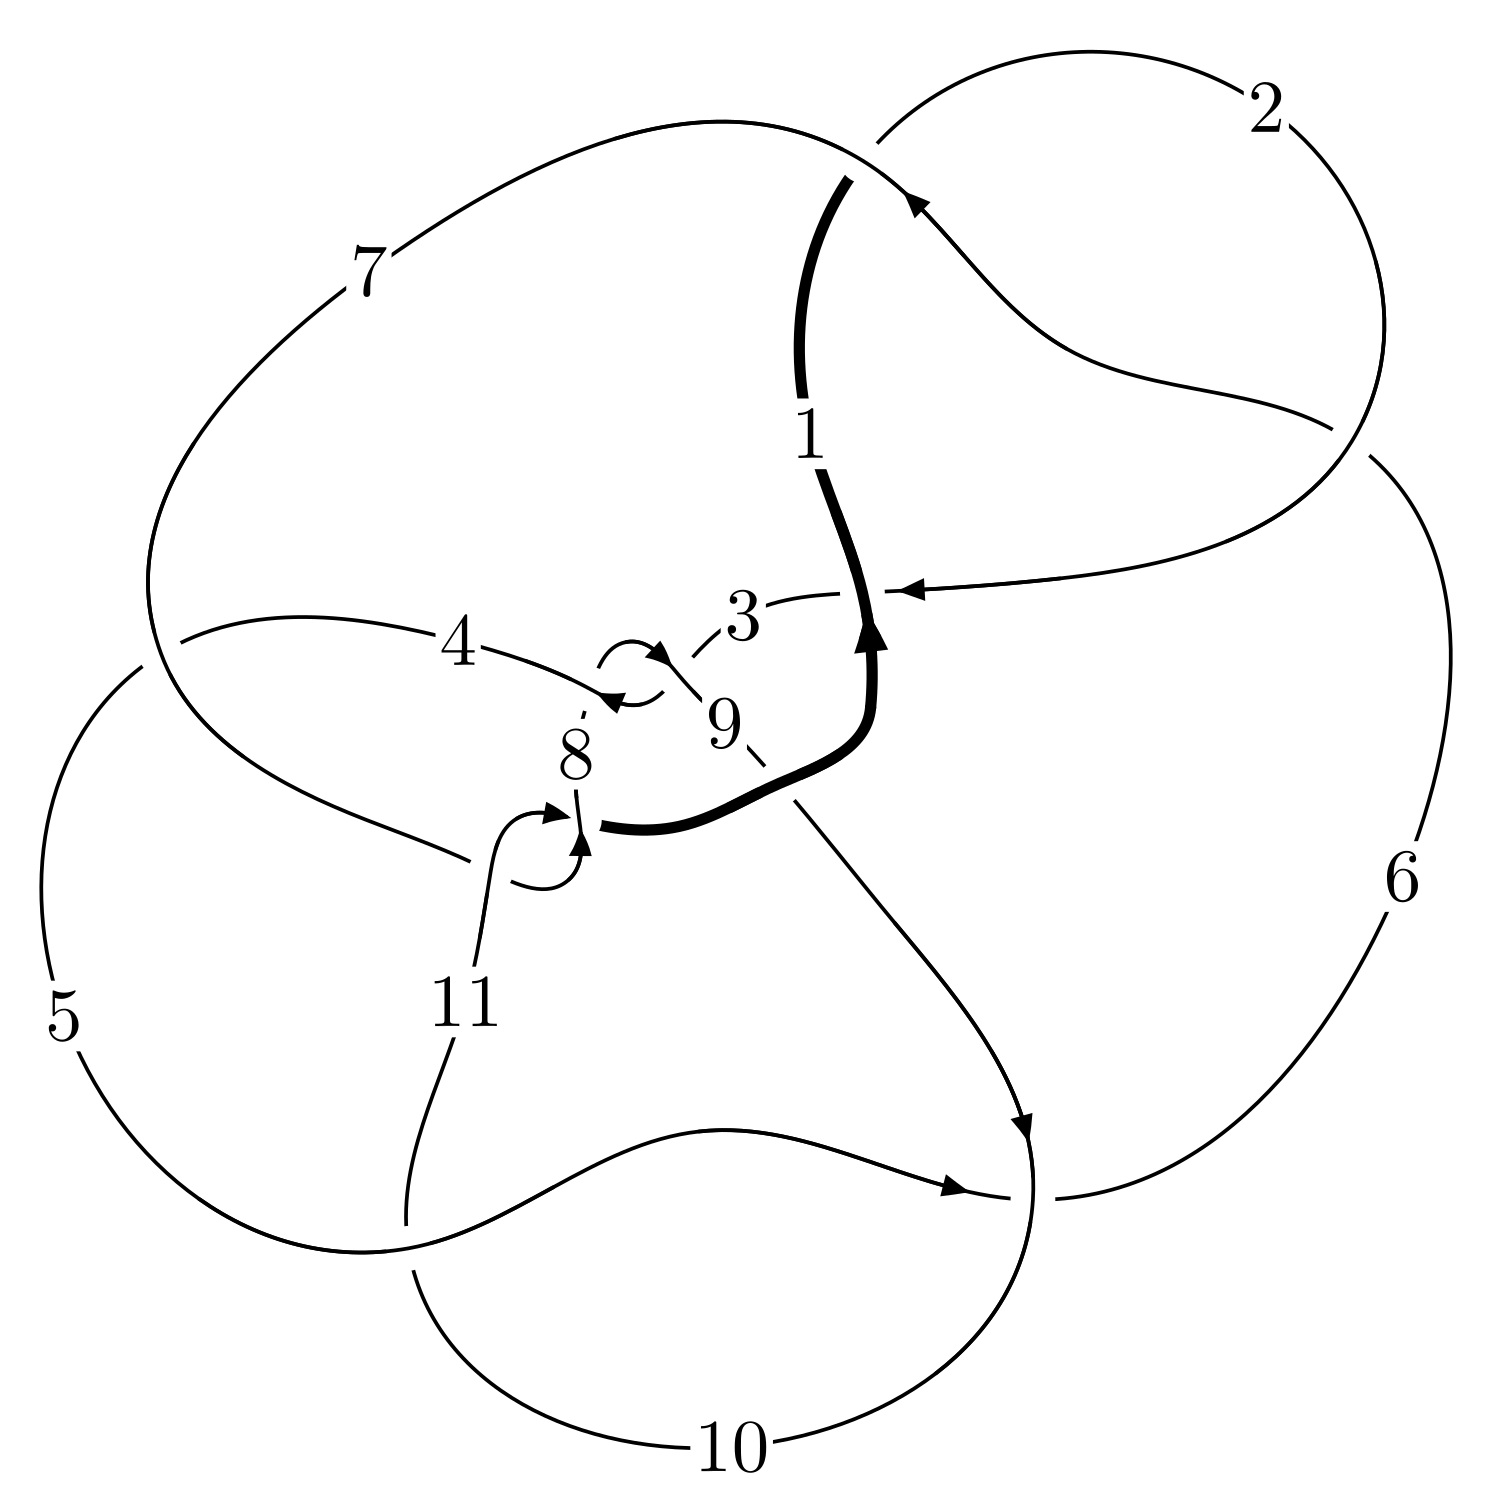
\includegraphics[width=112pt]{../../../GIT/diagram.site/Diagrams/png/738_11n_122.png}\\
\ \ \ A knot diagram\footnotemark}&
\allowdisplaybreaks
\textbf{Linearized knot diagam} \\
\cline{2-2}
 &
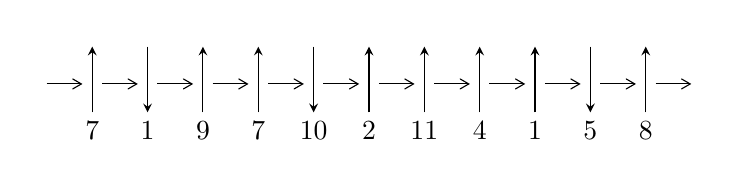
\begin{tikzpicture}[x=20pt, y=17pt]
	% nodes
	\node (C0) at (0, 0) {};
	\node (C1) at (1, 0) {};
	\node (C1U) at (1, +1) {};
	\node (C1D) at (1, -1) {7};

	\node (C2) at (2, 0) {};
	\node (C2U) at (2, +1) {};
	\node (C2D) at (2, -1) {1};

	\node (C3) at (3, 0) {};
	\node (C3U) at (3, +1) {};
	\node (C3D) at (3, -1) {9};

	\node (C4) at (4, 0) {};
	\node (C4U) at (4, +1) {};
	\node (C4D) at (4, -1) {7};

	\node (C5) at (5, 0) {};
	\node (C5U) at (5, +1) {};
	\node (C5D) at (5, -1) {10};

	\node (C6) at (6, 0) {};
	\node (C6U) at (6, +1) {};
	\node (C6D) at (6, -1) {2};

	\node (C7) at (7, 0) {};
	\node (C7U) at (7, +1) {};
	\node (C7D) at (7, -1) {11};

	\node (C8) at (8, 0) {};
	\node (C8U) at (8, +1) {};
	\node (C8D) at (8, -1) {4};

	\node (C9) at (9, 0) {};
	\node (C9U) at (9, +1) {};
	\node (C9D) at (9, -1) {1};

	\node (C10) at (10, 0) {};
	\node (C10U) at (10, +1) {};
	\node (C10D) at (10, -1) {5};

	\node (C11) at (11, 0) {};
	\node (C11U) at (11, +1) {};
	\node (C11D) at (11, -1) {8};
	\node (C12) at (12, 0) {};

	% arrows
	\draw[->,>={angle 60}]
	(C0) edge (C1) (C1) edge (C2) (C2) edge (C3) (C3) edge (C4) (C4) edge (C5) (C5) edge (C6) (C6) edge (C7) (C7) edge (C8) (C8) edge (C9) (C9) edge (C10) (C10) edge (C11) (C11) edge (C12) ;	\draw[->,>=stealth]
	(C1D) edge (C1U) (C2U) edge (C2D) (C3D) edge (C3U) (C4D) edge (C4U) (C5U) edge (C5D) (C6D) edge (C6U) (C7D) edge (C7U) (C8D) edge (C8U) (C9D) edge (C9U) (C10U) edge (C10D) (C11D) edge (C11U) ;
	\end{tikzpicture} \\
\hhline{~~} \\& 
\textbf{Solving Sequence} \\ \cline{2-2} 
 &
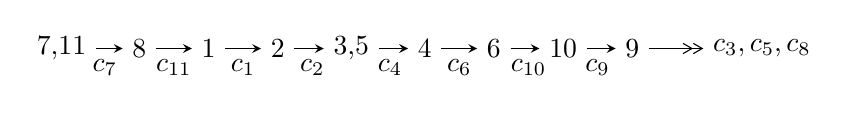
\begin{tikzpicture}[x=25pt, y=7pt]
	% node
	\node (A0) at (-1/8, 0) {7,11};
	\node (A1) at (1, 0) {8};
	\node (A2) at (2, 0) {1};
	\node (A3) at (3, 0) {2};
	\node (A4) at (65/16, 0) {3,5};
	\node (A5) at (41/8, 0) {4};
	\node (A6) at (49/8, 0) {6};
	\node (A7) at (57/8, 0) {10};
	\node (A8) at (65/8, 0) {9};
	\node (C1) at (1/2, -1) {$c_{7}$};
	\node (C2) at (3/2, -1) {$c_{11}$};
	\node (C3) at (5/2, -1) {$c_{1}$};
	\node (C4) at (7/2, -1) {$c_{2}$};
	\node (C5) at (37/8, -1) {$c_{4}$};
	\node (C6) at (45/8, -1) {$c_{6}$};
	\node (C7) at (53/8, -1) {$c_{10}$};
	\node (C8) at (61/8, -1) {$c_{9}$};
	\node (A9) at (10, 0) {$c_{3},c_{5},c_{8}$};

	% edge
	\draw[->,>=stealth]	
	(A0) edge (A1) (A1) edge (A2) (A2) edge (A3) (A3) edge (A4) (A4) edge (A5) (A5) edge (A6) (A6) edge (A7) (A7) edge (A8) ;
	\draw[->>,>={angle 60}]	
	(A8) edge (A9);
\end{tikzpicture} \\ 

\end{tabular} \\

\footnotetext{
The image of knot diagram is generated by the software ``\textbf{Draw programme}" developed by Andrew Bartholomew(\url{http://www.layer8.co.uk/maths/draw/index.htm\#Running-draw}), where we modified some parts for our purpose(\url{https://github.com/CATsTAILs/LinksPainter}).
}\phantom \\ \newline 
\centering \textbf{Ideals for irreducible components\footnotemark of $X_{\text{par}}$} 
 
\begin{align*}
I^u_{1}&=\langle 
u^{15}- u^{14}-5 u^{13}+5 u^{12}+7 u^{11}-9 u^{10}+7 u^9- u^8-25 u^7+17 u^6+9 u^5-7 u^4+17 u^3-13 u^2+4 b-2 u-4,\\
\phantom{I^u_{1}}&\phantom{= \langle  }- u^{15}+6 u^{13}+\cdots+4 a-4,\;u^{16}-2 u^{15}+\cdots+u+2\rangle \\
I^u_{2}&=\langle 
- u^4- u^3+u^2+b+u,\;- u^4+2 u^2+a-1,\;u^6-3 u^4+2 u^2+1\rangle \\
I^u_{3}&=\langle 
a^2+b,\;a^3+a-1,\;u+1\rangle \\
\\
\end{align*}
\raggedright * 3 irreducible components of $\dim_{\mathbb{C}}=0$, with total 25 representations.\\
\footnotetext{All coefficients of polynomials are rational numbers. But the coefficients are sometimes approximated in decimal forms when there is not enough margin.}
\newpage
\renewcommand{\arraystretch}{1}
\centering \section*{I. $I^u_{1}= \langle u^{15}- u^{14}+\cdots+4 b-4,\;- u^{15}+6 u^{13}+\cdots+4 a-4,\;u^{16}-2 u^{15}+\cdots+u+2 \rangle$}
\flushleft \textbf{(i) Arc colorings}\\
\begin{tabular}{m{7pt} m{180pt} m{7pt} m{180pt} }
\flushright $a_{7}=$&$\begin{pmatrix}1\\0\end{pmatrix}$ \\
\flushright $a_{11}=$&$\begin{pmatrix}0\\u\end{pmatrix}$ \\
\flushright $a_{8}=$&$\begin{pmatrix}1\\- u^2\end{pmatrix}$ \\
\flushright $a_{1}=$&$\begin{pmatrix}u\\- u^3+u\end{pmatrix}$ \\
\flushright $a_{2}=$&$\begin{pmatrix}- u^3+2 u\\- u^3+u\end{pmatrix}$ \\
\flushright $a_{3}=$&$\begin{pmatrix}u^7-2 u^5+2 u\\- u^9+3 u^7-3 u^5+u\end{pmatrix}$ \\
\flushright $a_{5}=$&$\begin{pmatrix}\frac{1}{4} u^{15}-\frac{3}{2} u^{13}+\cdots-\frac{9}{4} u+1\\-\frac{1}{4} u^{15}+\frac{1}{4} u^{14}+\cdots+\frac{1}{2} u+1\end{pmatrix}$ \\
\flushright $a_{4}=$&$\begin{pmatrix}\frac{1}{2} u^{15}-\frac{1}{4} u^{14}+\cdots+\frac{1}{4} u^2-\frac{11}{4} u\\-\frac{1}{4} u^{15}+\frac{1}{4} u^{14}+\cdots+\frac{1}{2} u+1\end{pmatrix}$ \\
\flushright $a_{6}=$&$\begin{pmatrix}u^6-3 u^4+2 u^2+1\\u^6-2 u^4+u^2\end{pmatrix}$ \\
\flushright $a_{10}=$&$\begin{pmatrix}\frac{1}{4} u^{13}-\frac{5}{4} u^{11}+\cdots+\frac{3}{4} u+1\\\frac{1}{2} u^{10}-2 u^8+\cdots-\frac{5}{2} u^2+\frac{1}{2} u\end{pmatrix}$ \\
\flushright $a_{9}=$&$\begin{pmatrix}-\frac{1}{2} u^{15}+\frac{1}{4} u^{14}+\cdots+\frac{7}{4} u+2\\\frac{1}{2} u^{15}-\frac{1}{2} u^{14}+\cdots-\frac{1}{4} u-\frac{1}{2}\end{pmatrix}$\\ \flushright $a_{9}=$&$\begin{pmatrix}-\frac{1}{2} u^{15}+\frac{1}{4} u^{14}+\cdots+\frac{7}{4} u+2\\\frac{1}{2} u^{15}-\frac{1}{2} u^{14}+\cdots-\frac{1}{4} u-\frac{1}{2}\end{pmatrix}$\\&\end{tabular}
\flushleft \textbf{(ii) Obstruction class $= -1$}\\~\\
\flushleft \textbf{(iii) Cusp Shapes $= -2 u^{15}+12 u^{13}-2 u^{12}-28 u^{11}+10 u^{10}+20 u^9-18 u^8+28 u^7+10 u^6-52 u^5+6 u^4+10 u^3-6 u^2+16 u+10$}\\~\\
\newpage\renewcommand{\arraystretch}{1}
\flushleft \textbf{(iv) u-Polynomials at the component}\newline \\
\begin{tabular}{m{50pt}|m{274pt}}
Crossings & \hspace{64pt}u-Polynomials at each crossing \\
\hline $$\begin{aligned}c_{1},c_{6}\end{aligned}$$&$\begin{aligned}
&u^{16}+3 u^{15}+\cdots-163 u+62
\end{aligned}$\\
\hline $$\begin{aligned}c_{2}\end{aligned}$$&$\begin{aligned}
&u^{16}+29 u^{15}+\cdots+16707 u+3844
\end{aligned}$\\
\hline $$\begin{aligned}c_{3},c_{8}\end{aligned}$$&$\begin{aligned}
&u^{16}- u^{15}+\cdots+14 u+5
\end{aligned}$\\
\hline $$\begin{aligned}c_{4}\end{aligned}$$&$\begin{aligned}
&u^{16}+5 u^{15}+\cdots-6 u+67
\end{aligned}$\\
\hline $$\begin{aligned}c_{5},c_{10}\end{aligned}$$&$\begin{aligned}
&u^{16}- u^{15}+\cdots+8 u+5
\end{aligned}$\\
\hline $$\begin{aligned}c_{7},c_{11}\end{aligned}$$&$\begin{aligned}
&u^{16}+2 u^{15}+\cdots- u+2
\end{aligned}$\\
\hline $$\begin{aligned}c_{9}\end{aligned}$$&$\begin{aligned}
&u^{16}- u^{15}+\cdots-2824 u+1117
\end{aligned}$\\
\hline
\end{tabular}\\~\\
\newpage\renewcommand{\arraystretch}{1}
\flushleft \textbf{(v) Riley Polynomials at the component}\newline \\
\begin{tabular}{m{50pt}|m{274pt}}
Crossings & \hspace{64pt}Riley Polynomials at each crossing \\
\hline $$\begin{aligned}c_{1},c_{6}\end{aligned}$$&$\begin{aligned}
&y^{16}+29 y^{15}+\cdots+16707 y+3844
\end{aligned}$\\
\hline $$\begin{aligned}c_{2}\end{aligned}$$&$\begin{aligned}
&y^{16}-75 y^{15}+\cdots+939185823 y+14776336
\end{aligned}$\\
\hline $$\begin{aligned}c_{3},c_{8}\end{aligned}$$&$\begin{aligned}
&y^{16}+27 y^{15}+\cdots-96 y+25
\end{aligned}$\\
\hline $$\begin{aligned}c_{4}\end{aligned}$$&$\begin{aligned}
&y^{16}+19 y^{15}+\cdots+15374 y+4489
\end{aligned}$\\
\hline $$\begin{aligned}c_{5},c_{10}\end{aligned}$$&$\begin{aligned}
&y^{16}- y^{15}+\cdots-64 y+25
\end{aligned}$\\
\hline $$\begin{aligned}c_{7},c_{11}\end{aligned}$$&$\begin{aligned}
&y^{16}-12 y^{15}+\cdots+19 y+4
\end{aligned}$\\
\hline $$\begin{aligned}c_{9}\end{aligned}$$&$\begin{aligned}
&y^{16}+51 y^{15}+\cdots-7186374 y+1247689
\end{aligned}$\\
\hline
\end{tabular}\\~\\
\newpage\flushleft \textbf{(vi) Complex Volumes and Cusp Shapes}
$$\begin{array}{c|c|c}  
\text{Solutions to }I^u_{1}& \I (\text{vol} + \sqrt{-1}CS) & \text{Cusp shape}\\
 \hline 
\begin{aligned}
u &= \phantom{-}0.077517 + 1.005540 I \\
a &= -1.07927 - 1.29543 I \\
b &= -0.62616 - 1.56703 I\end{aligned}
 & -15.2325 + 4.4644 I & \phantom{-}1.08918 - 2.21387 I \\ \hline\begin{aligned}
u &= \phantom{-}0.077517 - 1.005540 I \\
a &= -1.07927 + 1.29543 I \\
b &= -0.62616 + 1.56703 I\end{aligned}
 & -15.2325 - 4.4644 I & \phantom{-}1.08918 + 2.21387 I \\ \hline\begin{aligned}
u &= \phantom{-}0.170392 + 0.771288 I \\
a &= -0.408921 + 1.021250 I \\
b &= -0.482279 + 1.104540 I\end{aligned}
 & -4.05827 - 0.49300 I & -0.617664 + 0.214534 I \\ \hline\begin{aligned}
u &= \phantom{-}0.170392 - 0.771288 I \\
a &= -0.408921 - 1.021250 I \\
b &= -0.482279 - 1.104540 I\end{aligned}
 & -4.05827 + 0.49300 I & -0.617664 - 0.214534 I \\ \hline\begin{aligned}
u &= \phantom{-}1.160690 + 0.407151 I \\
a &= \phantom{-}0.600692 - 0.658208 I \\
b &= -1.126220 - 0.798721 I\end{aligned}
 & -1.06445 + 4.80370 I & \phantom{-}3.93778 - 5.08204 I \\ \hline\begin{aligned}
u &= \phantom{-}1.160690 - 0.407151 I \\
a &= \phantom{-}0.600692 + 0.658208 I \\
b &= -1.126220 + 0.798721 I\end{aligned}
 & -1.06445 - 4.80370 I & \phantom{-}3.93778 + 5.08204 I \\ \hline\begin{aligned}
u &= \phantom{-}1.293170 + 0.155822 I \\
a &= -0.056229 + 0.786374 I \\
b &= \phantom{-}0.86906 + 1.53568 I\end{aligned}
 & \phantom{-}5.01976 + 2.82849 I & \phantom{-}13.14002 - 4.04275 I \\ \hline\begin{aligned}
u &= \phantom{-}1.293170 - 0.155822 I \\
a &= -0.056229 - 0.786374 I \\
b &= \phantom{-}0.86906 - 1.53568 I\end{aligned}
 & \phantom{-}5.01976 - 2.82849 I & \phantom{-}13.14002 + 4.04275 I \\ \hline\begin{aligned}
u &= \phantom{-}1.269320 + 0.545322 I \\
a &= -1.162000 - 0.309874 I \\
b &= -0.241796 + 0.780806 I\end{aligned}
 & -11.56800 + 1.02407 I & \phantom{-}3.53875 - 0.89724 I \\ \hline\begin{aligned}
u &= \phantom{-}1.269320 - 0.545322 I \\
a &= -1.162000 + 0.309874 I \\
b &= -0.241796 - 0.780806 I\end{aligned}
 & -11.56800 - 1.02407 I & \phantom{-}3.53875 + 0.89724 I\\
 \hline 
 \end{array}$$\newpage$$\begin{array}{c|c|c}  
\text{Solutions to }I^u_{1}& \I (\text{vol} + \sqrt{-1}CS) & \text{Cusp shape}\\
 \hline 
\begin{aligned}
u &= -1.374820 + 0.254049 I \\
a &= -0.397419 - 0.220831 I \\
b &= \phantom{-}0.02694 - 1.60521 I\end{aligned}
 & \phantom{-}0.90149 - 3.13168 I & \phantom{-}3.23299 + 2.68195 I \\ \hline\begin{aligned}
u &= -1.374820 - 0.254049 I \\
a &= -0.397419 + 0.220831 I \\
b &= \phantom{-}0.02694 + 1.60521 I\end{aligned}
 & \phantom{-}0.90149 + 3.13168 I & \phantom{-}3.23299 - 2.68195 I \\ \hline\begin{aligned}
u &= -1.37116 + 0.47203 I \\
a &= \phantom{-}0.424287 + 1.067010 I \\
b &= -1.31943 + 2.03484 I\end{aligned}
 & -10.6907 - 9.7305 I & \phantom{-}4.40505 + 4.74516 I \\ \hline\begin{aligned}
u &= -1.37116 - 0.47203 I \\
a &= \phantom{-}0.424287 - 1.067010 I \\
b &= -1.31943 - 2.03484 I\end{aligned}
 & -10.6907 + 9.7305 I & \phantom{-}4.40505 - 4.74516 I \\ \hline\begin{aligned}
u &= -0.225111 + 0.325313 I \\
a &= \phantom{-}1.32887 - 1.40325 I \\
b &= \phantom{-}0.399881 - 0.330960 I\end{aligned}
 & \phantom{-}0.504151 - 0.997325 I & \phantom{-}7.27390 + 6.88407 I \\ \hline\begin{aligned}
u &= -0.225111 - 0.325313 I \\
a &= \phantom{-}1.32887 + 1.40325 I \\
b &= \phantom{-}0.399881 + 0.330960 I\end{aligned}
 & \phantom{-}0.504151 + 0.997325 I & \phantom{-}7.27390 - 6.88407 I\\
 \hline 
 \end{array}$$\newpage\newpage\renewcommand{\arraystretch}{1}
\centering \section*{II. $I^u_{2}= \langle - u^4- u^3+u^2+b+u,\;- u^4+2 u^2+a-1,\;u^6-3 u^4+2 u^2+1 \rangle$}
\flushleft \textbf{(i) Arc colorings}\\
\begin{tabular}{m{7pt} m{180pt} m{7pt} m{180pt} }
\flushright $a_{7}=$&$\begin{pmatrix}1\\0\end{pmatrix}$ \\
\flushright $a_{11}=$&$\begin{pmatrix}0\\u\end{pmatrix}$ \\
\flushright $a_{8}=$&$\begin{pmatrix}1\\- u^2\end{pmatrix}$ \\
\flushright $a_{1}=$&$\begin{pmatrix}u\\- u^3+u\end{pmatrix}$ \\
\flushright $a_{2}=$&$\begin{pmatrix}- u^3+2 u\\- u^3+u\end{pmatrix}$ \\
\flushright $a_{3}=$&$\begin{pmatrix}u^5-2 u^3+u\\- u^5+u^3+u\end{pmatrix}$ \\
\flushright $a_{5}=$&$\begin{pmatrix}u^4-2 u^2+1\\u^4+u^3- u^2- u\end{pmatrix}$ \\
\flushright $a_{4}=$&$\begin{pmatrix}- u^3- u^2+u+1\\u^4+u^3- u^2- u\end{pmatrix}$ \\
\flushright $a_{6}=$&$\begin{pmatrix}0\\u^4- u^2-1\end{pmatrix}$ \\
\flushright $a_{10}=$&$\begin{pmatrix}u^5-3 u^3+2 u\\u^5+u^4-2 u^3-2 u^2+u\end{pmatrix}$ \\
\flushright $a_{9}=$&$\begin{pmatrix}- u^4- u^3+2 u^2+2 u+1\\u^5+u^4-2 u^3-3 u^2\end{pmatrix}$\\ \flushright $a_{9}=$&$\begin{pmatrix}- u^4- u^3+2 u^2+2 u+1\\u^5+u^4-2 u^3-3 u^2\end{pmatrix}$\\&\end{tabular}
\flushleft \textbf{(ii) Obstruction class $= 1$}\\~\\
\flushleft \textbf{(iii) Cusp Shapes $= -4 u^4+8 u^2+4$}\\~\\
\newpage\renewcommand{\arraystretch}{1}
\flushleft \textbf{(iv) u-Polynomials at the component}\newline \\
\begin{tabular}{m{50pt}|m{274pt}}
Crossings & \hspace{64pt}u-Polynomials at each crossing \\
\hline $$\begin{aligned}c_{1},c_{6}\end{aligned}$$&$\begin{aligned}
&u^6+u^4+2 u^2+1
\end{aligned}$\\
\hline $$\begin{aligned}c_{2}\end{aligned}$$&$\begin{aligned}
&(u^3+u^2+2 u+1)^2
\end{aligned}$\\
\hline $$\begin{aligned}c_{3},c_{5},c_{8}\\c_{10}\end{aligned}$$&$\begin{aligned}
&(u^2+1)^3
\end{aligned}$\\
\hline $$\begin{aligned}c_{4}\end{aligned}$$&$\begin{aligned}
&u^6+4 u^5+11 u^4+10 u^3+8 u^2+2 u+1
\end{aligned}$\\
\hline $$\begin{aligned}c_{7},c_{11}\end{aligned}$$&$\begin{aligned}
&u^6-3 u^4+2 u^2+1
\end{aligned}$\\
\hline $$\begin{aligned}c_{9}\end{aligned}$$&$\begin{aligned}
&u^6-2 u^5- u^4+8 u^3+12 u^2+6 u+1
\end{aligned}$\\
\hline
\end{tabular}\\~\\
\newpage\renewcommand{\arraystretch}{1}
\flushleft \textbf{(v) Riley Polynomials at the component}\newline \\
\begin{tabular}{m{50pt}|m{274pt}}
Crossings & \hspace{64pt}Riley Polynomials at each crossing \\
\hline $$\begin{aligned}c_{1},c_{6}\end{aligned}$$&$\begin{aligned}
&(y^3+y^2+2 y+1)^2
\end{aligned}$\\
\hline $$\begin{aligned}c_{2}\end{aligned}$$&$\begin{aligned}
&(y^3+3 y^2+2 y-1)^2
\end{aligned}$\\
\hline $$\begin{aligned}c_{3},c_{5},c_{8}\\c_{10}\end{aligned}$$&$\begin{aligned}
&(y+1)^6
\end{aligned}$\\
\hline $$\begin{aligned}c_{4}\end{aligned}$$&$\begin{aligned}
&y^6+6 y^5+57 y^4+62 y^3+46 y^2+12 y+1
\end{aligned}$\\
\hline $$\begin{aligned}c_{7},c_{11}\end{aligned}$$&$\begin{aligned}
&(y^3-3 y^2+2 y+1)^2
\end{aligned}$\\
\hline $$\begin{aligned}c_{9}\end{aligned}$$&$\begin{aligned}
&y^6-6 y^5+57 y^4-62 y^3+46 y^2-12 y+1
\end{aligned}$\\
\hline
\end{tabular}\\~\\
\newpage\flushleft \textbf{(vi) Complex Volumes and Cusp Shapes}
$$\begin{array}{c|c|c}  
\text{Solutions to }I^u_{2}& \I (\text{vol} + \sqrt{-1}CS) & \text{Cusp shape}\\
 \hline 
\begin{aligned}
u &= \phantom{-}1.307140 + 0.215080 I \\
a &= \phantom{-}0.122561 + 0.744862 I \\
b &= \phantom{-}1.52978 + 2.18458 I\end{aligned}
 & \phantom{-}3.02413 + 2.82812 I & \phantom{-}7.50976 - 2.97945 I \\ \hline\begin{aligned}
u &= \phantom{-}1.307140 - 0.215080 I \\
a &= \phantom{-}0.122561 - 0.744862 I \\
b &= \phantom{-}1.52978 - 2.18458 I\end{aligned}
 & \phantom{-}3.02413 - 2.82812 I & \phantom{-}7.50976 + 2.97945 I \\ \hline\begin{aligned}
u &= -1.307140 + 0.215080 I \\
a &= \phantom{-}0.122561 - 0.744862 I \\
b &= \phantom{-}0.040058 - 0.429702 I\end{aligned}
 & \phantom{-}3.02413 - 2.82812 I & \phantom{-}7.50976 + 2.97945 I \\ \hline\begin{aligned}
u &= -1.307140 - 0.215080 I \\
a &= \phantom{-}0.122561 + 0.744862 I \\
b &= \phantom{-}0.040058 + 0.429702 I\end{aligned}
 & \phantom{-}3.02413 + 2.82812 I & \phantom{-}7.50976 - 2.97945 I \\ \hline\begin{aligned}
u &= \phantom{-0.000000 -}0.569840 I \\
a &= \phantom{-}1.75488\phantom{ +0.000000I} \\
b &= \phantom{-}0.430160 - 0.754878 I\end{aligned}
 & -1.11345\phantom{ +0.000000I} & \phantom{-}0.980490\phantom{ +0.000000I} \\ \hline\begin{aligned}
u &= \phantom{-0.000000 } -0.569840 I \\
a &= \phantom{-}1.75488\phantom{ +0.000000I} \\
b &= \phantom{-}0.430160 + 0.754878 I\end{aligned}
 & -1.11345\phantom{ +0.000000I} & \phantom{-}0.980490\phantom{ +0.000000I}\\
 \hline 
 \end{array}$$\newpage\newpage\renewcommand{\arraystretch}{1}
\centering \section*{III. $I^u_{3}= \langle a^2+b,\;a^3+a-1,\;u+1 \rangle$}
\flushleft \textbf{(i) Arc colorings}\\
\begin{tabular}{m{7pt} m{180pt} m{7pt} m{180pt} }
\flushright $a_{7}=$&$\begin{pmatrix}1\\0\end{pmatrix}$ \\
\flushright $a_{11}=$&$\begin{pmatrix}0\\-1\end{pmatrix}$ \\
\flushright $a_{8}=$&$\begin{pmatrix}1\\-1\end{pmatrix}$ \\
\flushright $a_{1}=$&$\begin{pmatrix}-1\\0\end{pmatrix}$ \\
\flushright $a_{2}=$&$\begin{pmatrix}-1\\0\end{pmatrix}$ \\
\flushright $a_{3}=$&$\begin{pmatrix}-1\\0\end{pmatrix}$ \\
\flushright $a_{5}=$&$\begin{pmatrix}a\\- a^2\end{pmatrix}$ \\
\flushright $a_{4}=$&$\begin{pmatrix}a^2+a\\- a^2\end{pmatrix}$ \\
\flushright $a_{6}=$&$\begin{pmatrix}1\\0\end{pmatrix}$ \\
\flushright $a_{10}=$&$\begin{pmatrix}- a^2\\- a\end{pmatrix}$ \\
\flushright $a_{9}=$&$\begin{pmatrix}- a^2+a\\- a\end{pmatrix}$\\ \flushright $a_{9}=$&$\begin{pmatrix}- a^2+a\\- a\end{pmatrix}$\\&\end{tabular}
\flushleft \textbf{(ii) Obstruction class $= -1$}\\~\\
\flushleft \textbf{(iii) Cusp Shapes $= 6$}\\~\\
\newpage\renewcommand{\arraystretch}{1}
\flushleft \textbf{(iv) u-Polynomials at the component}\newline \\
\begin{tabular}{m{50pt}|m{274pt}}
Crossings & \hspace{64pt}u-Polynomials at each crossing \\
\hline $$\begin{aligned}c_{1},c_{2},c_{6}\end{aligned}$$&$\begin{aligned}
&u^3
\end{aligned}$\\
\hline $$\begin{aligned}c_{3},c_{5},c_{8}\\c_{9},c_{10}\end{aligned}$$&$\begin{aligned}
&u^3+u-1
\end{aligned}$\\
\hline $$\begin{aligned}c_{4}\end{aligned}$$&$\begin{aligned}
&u^3-2 u^2+u+1
\end{aligned}$\\
\hline $$\begin{aligned}c_{7},c_{11}\end{aligned}$$&$\begin{aligned}
&(u-1)^3
\end{aligned}$\\
\hline
\end{tabular}\\~\\
\newpage\renewcommand{\arraystretch}{1}
\flushleft \textbf{(v) Riley Polynomials at the component}\newline \\
\begin{tabular}{m{50pt}|m{274pt}}
Crossings & \hspace{64pt}Riley Polynomials at each crossing \\
\hline $$\begin{aligned}c_{1},c_{2},c_{6}\end{aligned}$$&$\begin{aligned}
&y^3
\end{aligned}$\\
\hline $$\begin{aligned}c_{3},c_{5},c_{8}\\c_{9},c_{10}\end{aligned}$$&$\begin{aligned}
&y^3+2 y^2+y-1
\end{aligned}$\\
\hline $$\begin{aligned}c_{4}\end{aligned}$$&$\begin{aligned}
&y^3-2 y^2+5 y-1
\end{aligned}$\\
\hline $$\begin{aligned}c_{7},c_{11}\end{aligned}$$&$\begin{aligned}
&(y-1)^3
\end{aligned}$\\
\hline
\end{tabular}\\~\\
\newpage\flushleft \textbf{(vi) Complex Volumes and Cusp Shapes}
$$\begin{array}{c|c|c}  
\text{Solutions to }I^u_{3}& \I (\text{vol} + \sqrt{-1}CS) & \text{Cusp shape}\\
 \hline 
\begin{aligned}
u &= -1.00000\phantom{ +0.000000I} \\
a &= -0.341164 + 1.161540 I \\
b &= \phantom{-}1.23279 + 0.79255 I\end{aligned}
 & \phantom{-}1.64493\phantom{ +0.000000I} & \phantom{-}6.00000\phantom{ +0.000000I} \\ \hline\begin{aligned}
u &= -1.00000\phantom{ +0.000000I} \\
a &= -0.341164 - 1.161540 I \\
b &= \phantom{-}1.23279 - 0.79255 I\end{aligned}
 & \phantom{-}1.64493\phantom{ +0.000000I} & \phantom{-}6.00000\phantom{ +0.000000I} \\ \hline\begin{aligned}
u &= -1.00000\phantom{ +0.000000I} \\
a &= \phantom{-}0.682328\phantom{ +0.000000I} \\
b &= -0.465571\phantom{ +0.000000I}\end{aligned}
 & \phantom{-}1.64493\phantom{ +0.000000I} & \phantom{-}6.00000\phantom{ +0.000000I}\\
 \hline 
 \end{array}$$\newpage
\newpage\renewcommand{\arraystretch}{1}
\centering \section*{ IV. u-Polynomials}
\begin{tabular}{m{50pt}|m{274pt}}
Crossings & \hspace{64pt}u-Polynomials at each crossing \\
\hline $$\begin{aligned}c_{1},c_{6}\end{aligned}$$&$\begin{aligned}
&u^3(u^6+u^4+2 u^2+1)(u^{16}+3 u^{15}+\cdots-163 u+62)
\end{aligned}$\\
\hline $$\begin{aligned}c_{2}\end{aligned}$$&$\begin{aligned}
&u^3(u^3+u^2+2 u+1)^2(u^{16}+29 u^{15}+\cdots+16707 u+3844)
\end{aligned}$\\
\hline $$\begin{aligned}c_{3},c_{8}\end{aligned}$$&$\begin{aligned}
&((u^2+1)^3)(u^3+u-1)(u^{16}- u^{15}+\cdots+14 u+5)
\end{aligned}$\\
\hline $$\begin{aligned}c_{4}\end{aligned}$$&$\begin{aligned}
&(u^3-2 u^2+u+1)(u^6+4 u^5+11 u^4+10 u^3+8 u^2+2 u+1)\\
&\cdot(u^{16}+5 u^{15}+\cdots-6 u+67)
\end{aligned}$\\
\hline $$\begin{aligned}c_{5},c_{10}\end{aligned}$$&$\begin{aligned}
&((u^2+1)^3)(u^3+u-1)(u^{16}- u^{15}+\cdots+8 u+5)
\end{aligned}$\\
\hline $$\begin{aligned}c_{7},c_{11}\end{aligned}$$&$\begin{aligned}
&((u-1)^3)(u^6-3 u^4+2 u^2+1)(u^{16}+2 u^{15}+\cdots- u+2)
\end{aligned}$\\
\hline $$\begin{aligned}c_{9}\end{aligned}$$&$\begin{aligned}
&(u^3+u-1)(u^6-2 u^5- u^4+8 u^3+12 u^2+6 u+1)\\
&\cdot(u^{16}- u^{15}+\cdots-2824 u+1117)
\end{aligned}$\\
\hline
\end{tabular}\newpage\renewcommand{\arraystretch}{1}
\centering \section*{ V. Riley Polynomials}
\begin{tabular}{m{50pt}|m{274pt}}
Crossings & \hspace{64pt}Riley Polynomials at each crossing \\
\hline $$\begin{aligned}c_{1},c_{6}\end{aligned}$$&$\begin{aligned}
&y^3(y^3+y^2+2 y+1)^2(y^{16}+29 y^{15}+\cdots+16707 y+3844)
\end{aligned}$\\
\hline $$\begin{aligned}c_{2}\end{aligned}$$&$\begin{aligned}
&y^3(y^3+3 y^2+2 y-1)^2\\
&\cdot(y^{16}-75 y^{15}+\cdots+939185823 y+14776336)
\end{aligned}$\\
\hline $$\begin{aligned}c_{3},c_{8}\end{aligned}$$&$\begin{aligned}
&((y+1)^6)(y^3+2 y^2+y-1)(y^{16}+27 y^{15}+\cdots-96 y+25)
\end{aligned}$\\
\hline $$\begin{aligned}c_{4}\end{aligned}$$&$\begin{aligned}
&(y^3-2 y^2+5 y-1)(y^6+6 y^5+57 y^4+62 y^3+46 y^2+12 y+1)\\
&\cdot(y^{16}+19 y^{15}+\cdots+15374 y+4489)
\end{aligned}$\\
\hline $$\begin{aligned}c_{5},c_{10}\end{aligned}$$&$\begin{aligned}
&((y+1)^6)(y^3+2 y^2+y-1)(y^{16}- y^{15}+\cdots-64 y+25)
\end{aligned}$\\
\hline $$\begin{aligned}c_{7},c_{11}\end{aligned}$$&$\begin{aligned}
&((y-1)^3)(y^3-3 y^2+2 y+1)^2(y^{16}-12 y^{15}+\cdots+19 y+4)
\end{aligned}$\\
\hline $$\begin{aligned}c_{9}\end{aligned}$$&$\begin{aligned}
&(y^3+2 y^2+y-1)(y^6-6 y^5+57 y^4-62 y^3+46 y^2-12 y+1)\\
&\cdot(y^{16}+51 y^{15}+\cdots-7186374 y+1247689)
\end{aligned}$\\
\hline
\end{tabular}
\vskip 2pc
\end{document}